\documentclass[tikz,border=10pt]{standalone}
\begin{document}
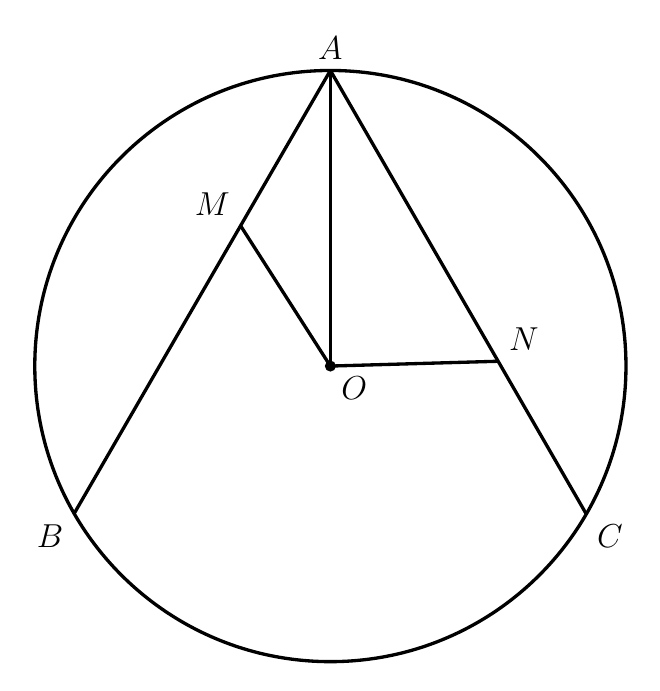
\begin{tikzpicture}[line join=round, line width=1.2pt]
% Named coordinates (cm). Scale s = 0.010596 cm/px, centred on circle centre (368.35,410.74), y flipped.
\coordinate (O) at (0,0);          % circle centre (px 368.00,410.34)
\coordinate (A) at (0,3.754);      % px (368.36,56.5)
\coordinate (B) at (-3.254,-1.873);% px (61.26,587.46)
\coordinate (C) at (3.250,-1.879); % px (675.08,588.08)
\coordinate (M) at (-1.139,1.780); % px (260.87,242.8)
\coordinate (N) at (2.132,0.061);  % px (569.55,405.0)

% Circle (radius 354.31 px)
\draw (O) circle[radius=3.754];

% Segments (BC intentionally omitted)
\draw (A) -- (B);   % passes through M
\draw (A) -- (C);   % passes through N
\draw (A) -- (O);   % vertical
\draw (O) -- (M);
\draw (O) -- (N);

% Filled dot at O
\fill (O) circle (2pt);

% Labels (font from style metrics)
\node[font=\fontsize{12.5}{15}\selectfont, above] at (A) {$A$};
\node[font=\fontsize{12.5}{15}\selectfont, below left] at (B) {$B$};
\node[font=\fontsize{12.5}{15}\selectfont, below right] at (C) {$C$};
\node[font=\fontsize{12.5}{15}\selectfont, above left] at (M) {$M$};
\node[font=\fontsize{12.5}{15}\selectfont, above right] at (N) {$N$};
\node[font=\fontsize{12.5}{15}\selectfont, below right] at (O) {$O$};
\end{tikzpicture}
\end{document}